\documentclass{standalone}

\usepackage{pgfplots,tikz,amsmath}
\begin{document}
        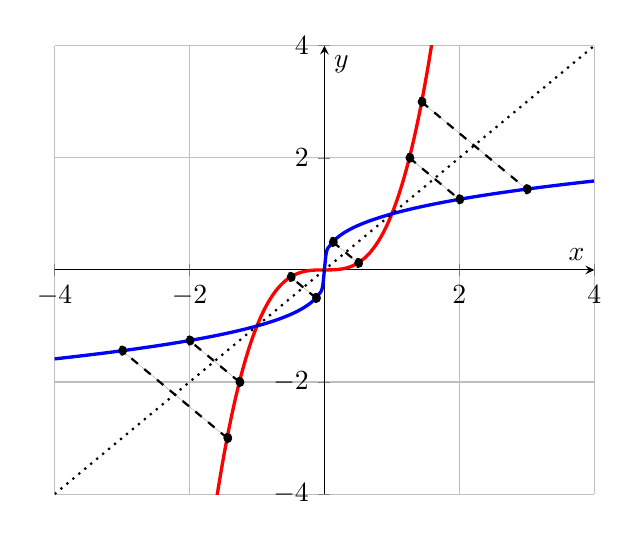
\begin{tikzpicture}
            \begin{axis}[axis lines=center, xlabel={$x$}, ylabel={$y$}, domain=-4:4,
                ymin=-4, ymax=4, xmin=-4, xmax=4, grid]
                \addplot[smooth, very thick, red, samples=150] {x^3};
                \addplot[smooth, very thick, blue, samples=150] {(x/abs(x))*abs(x)^(1/3)};
                \draw[dashed, thick, fill=black] (axis cs:1.26,2) circle(0.05cm) -- (axis
                cs:2,1.26) circle(0.05cm);
                \draw[dashed, thick, fill=black] (axis cs:-1.26,-2) circle(0.05cm) -- (axis
                cs:-2,-1.26) circle(0.05cm);
                \draw[dashed, thick, fill=black] (axis cs:-0.125,-.5) circle(0.05cm) -- (axis
                cs:-0.5,-0.125) circle(0.05cm);
                \draw[dashed, thick, fill=black] (axis cs:0.125,.5) circle(0.05cm) -- (axis
                cs:0.5,0.125) circle(0.05cm);
                \draw[dashed, thick, fill=black] (axis cs:1.44,3) circle(0.05cm) -- (axis
                cs:3,1.44) circle(0.05cm);
                \draw[dashed, thick, fill=black] (axis cs:-1.44,-3) circle(0.05cm) -- (axis
                cs:-3,-1.44) circle(0.05cm);
                \addplot[smooth, black, dotted, thick] {x};
            \end{axis}
        \end{tikzpicture}
\end{document}
